\documentclass{iansnotes}

\title{Qubits}
\author{ian.mcloughlin@atu.ie}
\date{Last updated: \today}

\begin{document}
 
\maketitle


\section{Matrices}

$\begin{bmatrix} \alpha \\ \beta \end{bmatrix} = \alpha \begin{bmatrix} 1 \\ 0 \end{bmatrix} + \beta \begin{bmatrix} 0 \\ 1 \end{bmatrix}$


\vspace{10mm}

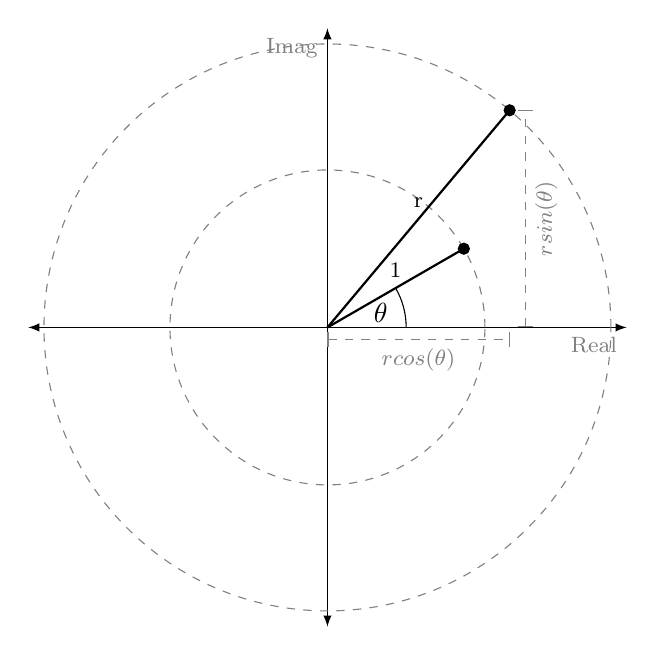
\begin{tikzpicture}[scale=2]
  % X axis
  \draw[latex-latex] (-1.9, 0) -- (1.9, 0) node[below left, gray] {\footnotesize Real};
  % Y axis
  \draw[latex-latex] (0, -1.9) -- (0, 1.9) node[below left, gray] {\footnotesize Imag};

  % Unit circle.
  \draw[gray, dashed] (0, 0) circle (1);
  % Outer circle.
  \draw[gray, dashed] (0, 0) circle (1.8);

  % Unit complex number magnitude.
  \draw[-, thick] (0, 0) --node[above] {\footnotesize 1} (30:1);
  % Dot for complex number.
  \draw[fill=black] (30:1) circle (1pt);
  % Projection of point onto x.
  %\draw[dashed] (30:1) -- ++(0,{-sin(30)});
  % Cos theta.
  %\draw[gray, |-|, dashed] (0, -0.075) --node[below] {\footnotesize $cos(\theta)$} ({cos(30)}, -0.075);
  % Sin theta.
  %\draw[gray, |-|, dashed] ({cos(30) + 0.1}, 0) --node[below, rotate=90] {\footnotesize $sin(\theta)$} ({cos(30) + 0.1}, {sin(30)});

  % Another complex number magnitude.
  \draw[-, thick] (0, 0) --node[above=0.25] {\footnotesize r} (50:1.8);
  % Dot for complex number.
  \draw[fill=black] (50:1.8) circle (1pt);

  % Cos theta.
  \draw[gray, |-|, dashed] (0, -0.075) --node[below] {\footnotesize $r cos(\theta)$} ({1.8 * cos(50)}, -0.075);
  % Sin theta.
  \draw[gray, |-|, dashed] ({1.8 * cos(50) + 0.1}, 0) --node[below, rotate=90] {\footnotesize $r sin(\theta)$} ({1.8 * cos(50) + 0.1}, {1.8 * sin(50)});


  \draw (0:0.5) arc (0:30:0.5);
  \path (15:0.35) node {$\theta$};


\end{tikzpicture}







\end{document}